\subsection{Process View}
\label{sec:processView}
The purpose of the Process View is to give the customer an overview of how some
of the main functionality has been implemented. We have chosen to do this
through Sequence Diagrams. These diagrams shows the main data flow of the system.

We have chosen to include the following functionality:
\begin{itemize}
	\item Medication completed
	\item Change of childrens health status
\end{itemize}



\subsubsection{Medication Completed}
\begin{figure}[h!]
	\centering
		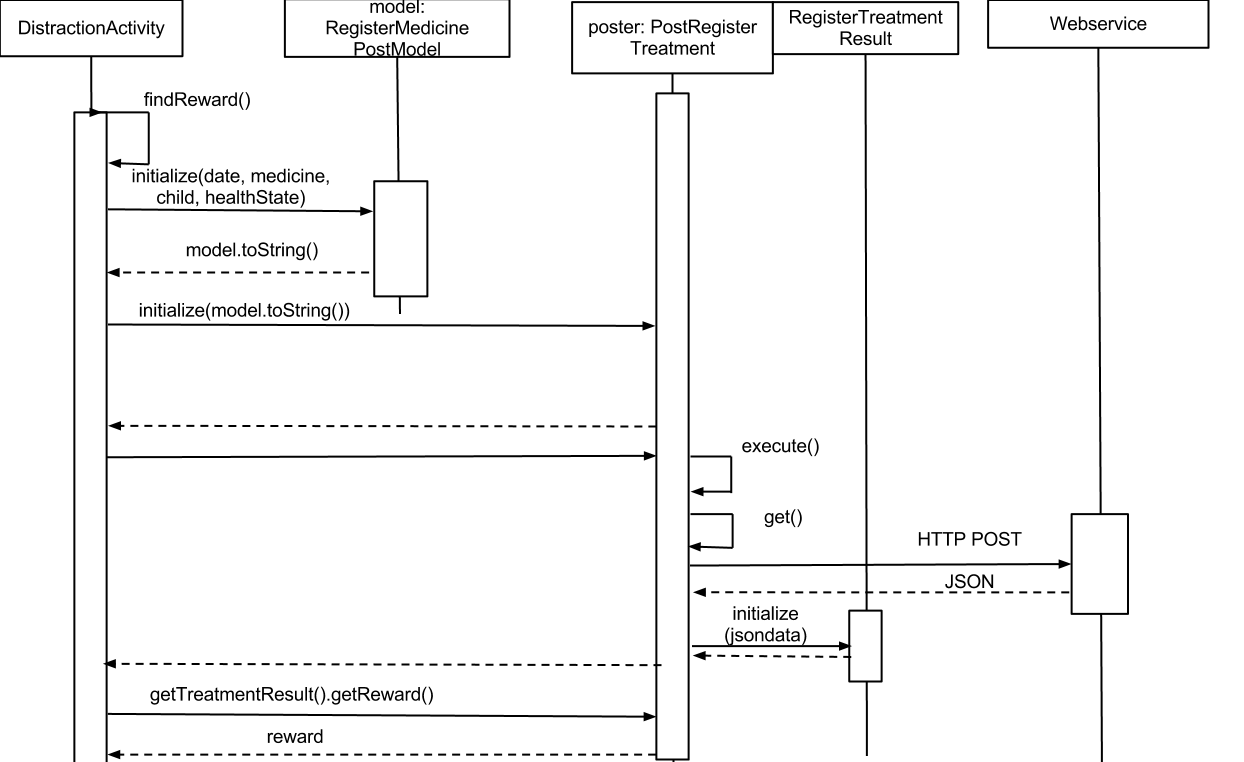
\includegraphics[width = 17.5 cm]{Pictures/ArchPictures/gapparchpictures/medication_finished.png}
	\caption{Sequence diagram for medication completed}
	\label{fig:seq-diagram-medication}
\end{figure}

Figure \ref{fig:seq-diagram-medication} shows a sequence diagram for the event of a medication completed. 
When a medication is completed, \code{DistractionActivity} creates a new instance of \code{RegisterMedicinePostModel}, before it uses this instance's \code{toString()} method to 
create an instance of \code{PostRegisterTreatment}. This poster does an HTTP POST to ``register\_medicine\_taken.php'', which 
in turn updates the databse. The webservice then returns JSON-formatted data, with the reward included. \code{RegisterMedicinePostModel} 
interprets the returned data, and stores the reward in a private variable, which the \code{DistractionActivity} in turn accesses to show the 
child the reward collected from the treatment.

\subsubsection{Change Of Childrens Health Status}
\begin{figure}[h!]
	\centering
		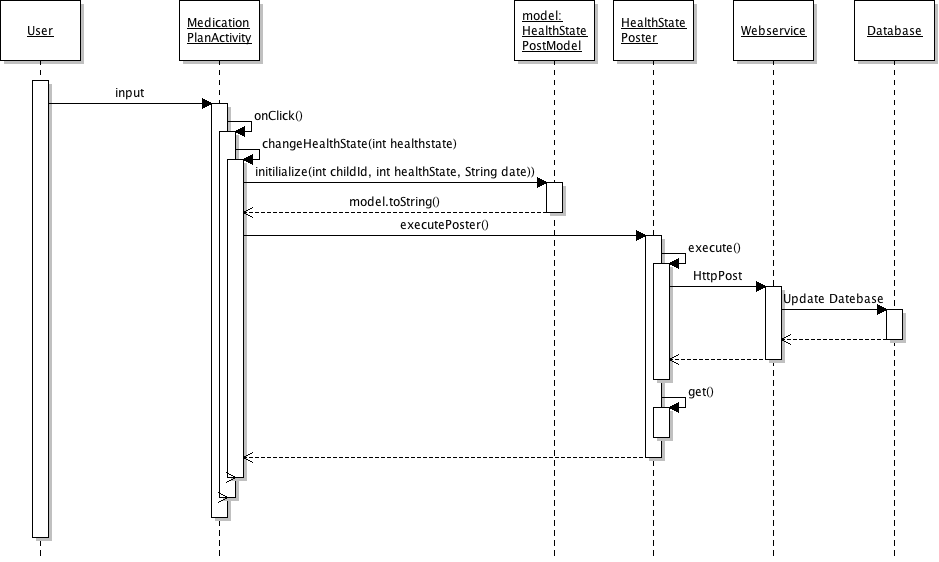
\includegraphics[width = 17.5 cm]{Pictures/ArchPictures/gapparchpictures/sequence_health_state.png}
	\caption{Sequence diagram for changing medication plan}
	\label{fig:seq-diagram-healthstate}
\end{figure}
Figure \ref{fig:seq-diagram-healthstate} shows a sequence diagram for the event of changing
a child's health status. The user gives input on one of three checkboxes that \code{MedicationPlanActivity} receives. The activity then calls creates 
a new instance of \code{HealthStatePostModel}, and uses this model's \code{toString()} to execute \code{HealthStatePoster}. \code{HealthStatePoster} makes an HTTP POST to ``set\_child\_state.php'' with 
appropriate POST parameters. The webservice updates the database, before it returns JSON-formatted data to the \code{HealthStatePoster}.

\subsubsection{Notification and medication on Karotz}
\begin{figure}
	\centering
		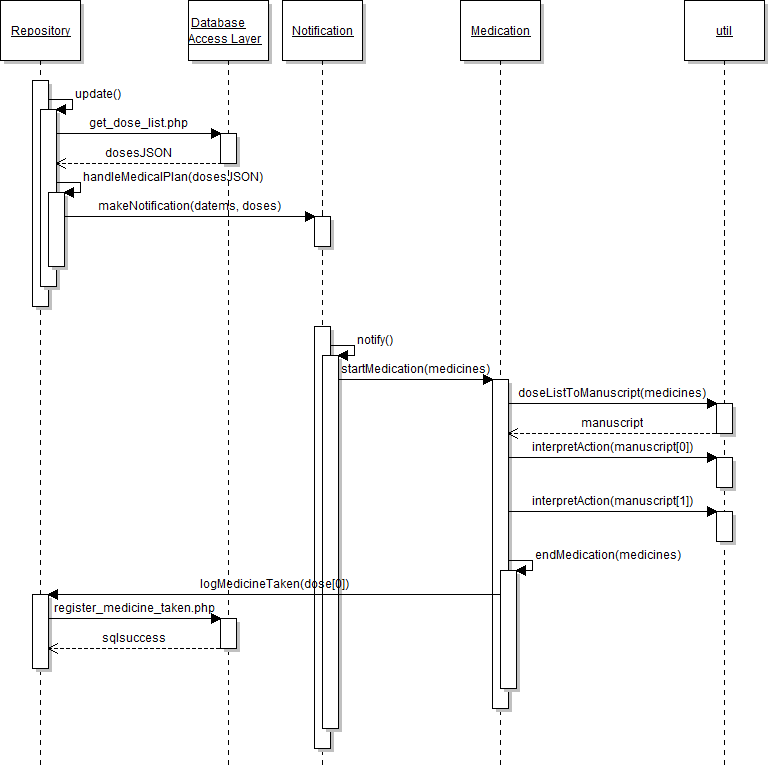
\includegraphics[width=\linewidth]{Pictures/ArchPictures/KarotzMedicationSequence}
	\caption{Sequence diagram for notification and medication on Karotz}
	\label{fig:karotz-sequence}
\end{figure}
Figure \ref{fig:karotz-sequence} shows a sequence diagram for notification and medication on the Karotz. The Karotz routinely updates itself by
calling a get function on the database access layer. The \code{Repository} object requests that a new notification event is made for the closest
medicine dose that should be taken. When the timeout is done, \code{Notification} calls \code{startMedication()} in \code{Medication} in order
to start a sequence of events that makes up the distraction sequence. This sequence is represented as a list of actions---called a \emph{manuscript}.
The manuscript is interpreted by the \code{util} module which creates and runs a function based on a premade specification. Each action contains
an url to a sound file, and an activator which represents how the next action in the manuscript is triggered. The manuscript is detailed further in
Appendix \ref{apx:karotzManuscript}. When each action in the manuscript is completed, the \code{Medication} module calls \code{logMedicineTaken()}
in \code{Repository} once for each dose, and the database is thus updated with the registered medicines.

